\section{Design}

CLAS12 Trigger System is designed as 3-stage pipeline-style system with total latency up to 8us. Stage 1 receives information from various CLAS12 detecrors and performs data processing in according to the type of detector. Stage 2 performs timing and geometry coincidence between different subset of detectors in 6 groups corresponding to 6-sector CLAS12 detector structure, as well as coincidence with information from central detectors. Stage 3 forms final trigger decision.
CLAS12 Trigger diagram is shown on Fig.~\ref{fig:TriggerDiagram}.

\begin{figure}[hbt]
	\centering
	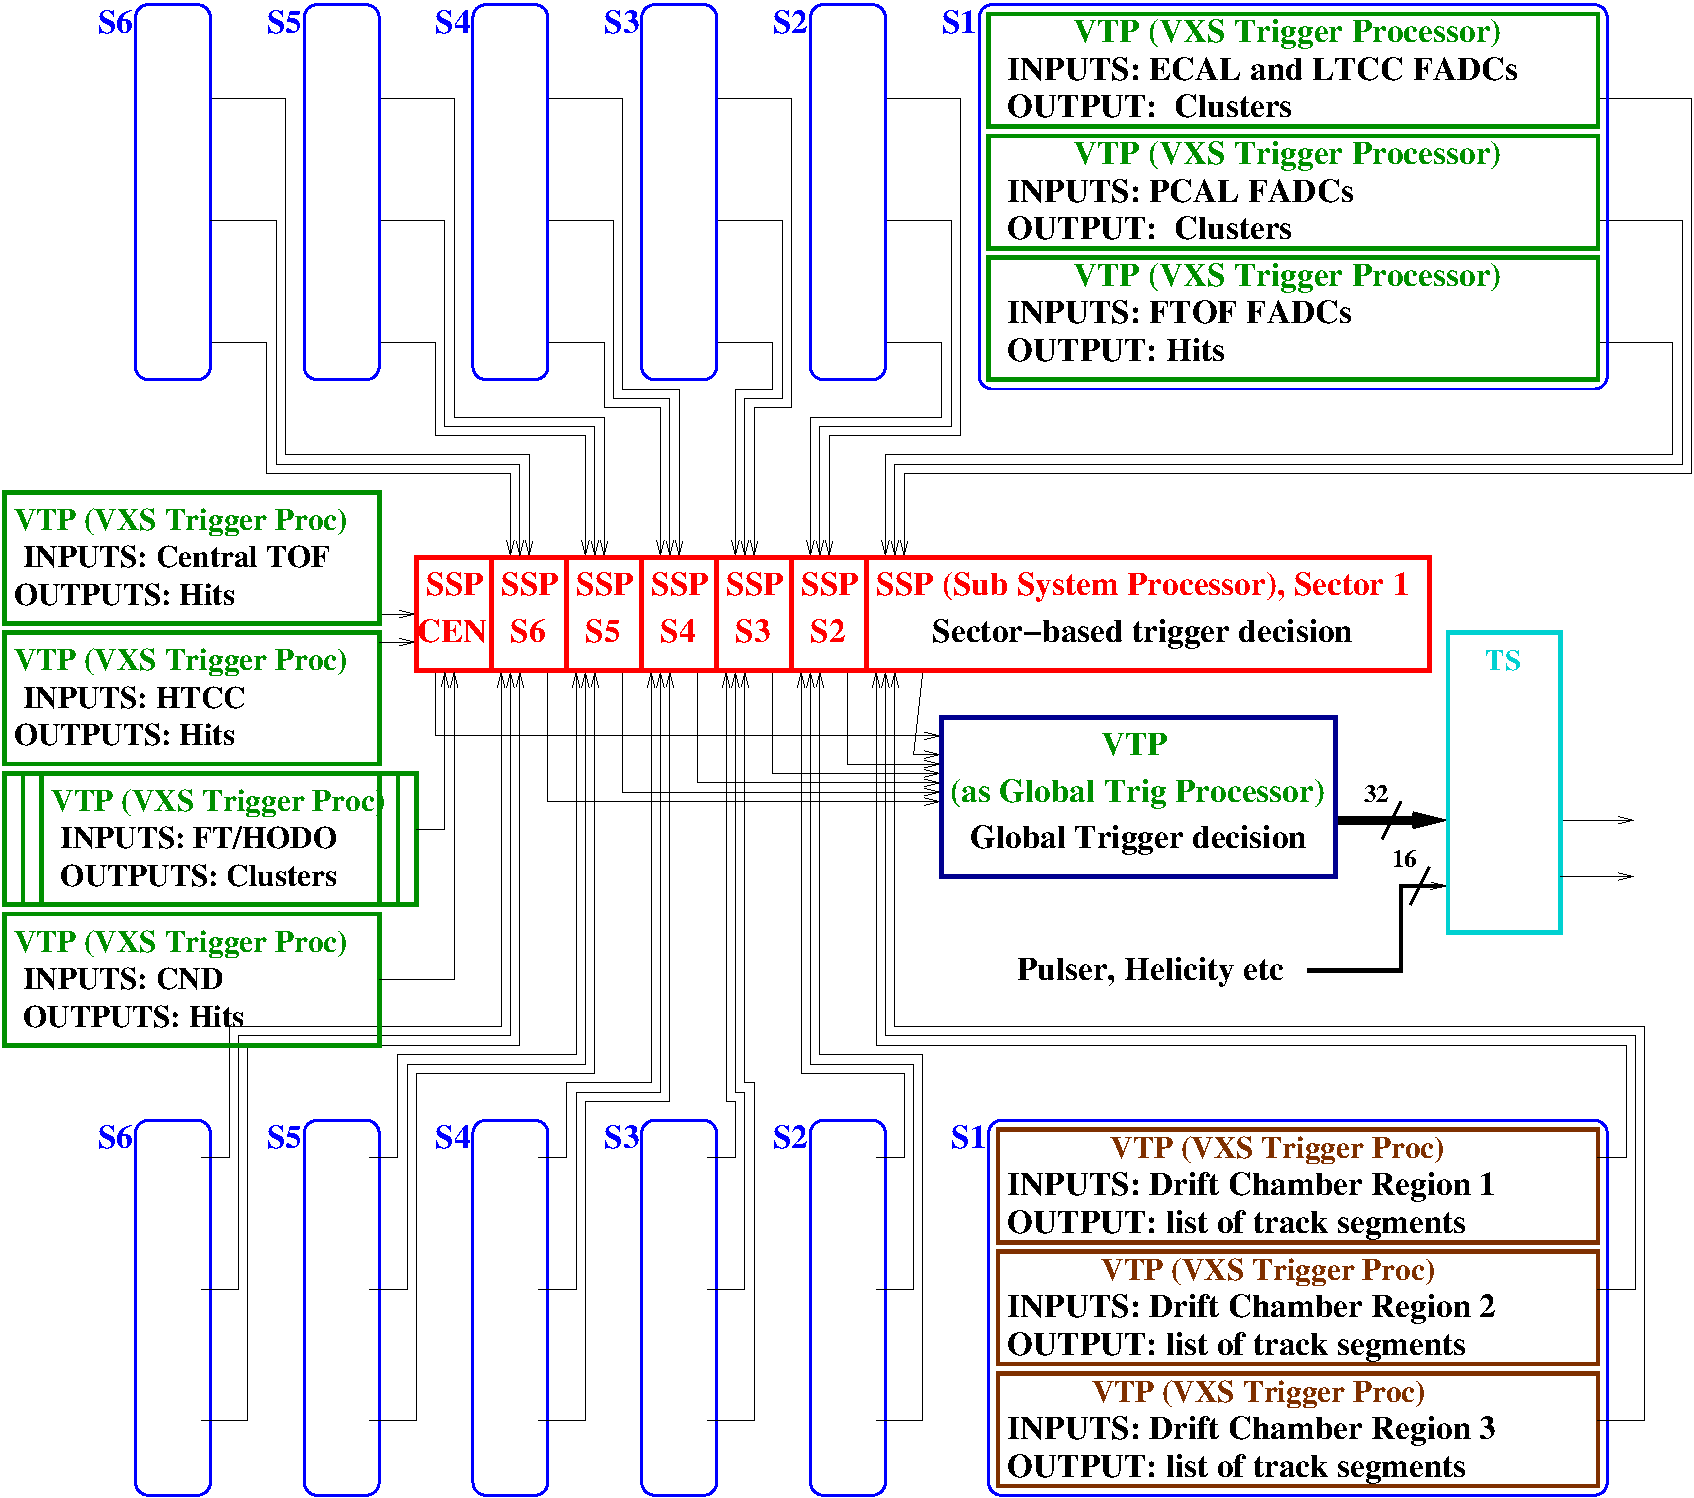
\includegraphics[width=1.0\columnwidth,keepaspectratio]{img/CLAS12_TRIGGER_1.pdf}
	\caption{CLAS12 Trigger System Diagram}
	\label{fig:TriggerDiagram}
\end{figure}


\subsection{Stage 1} The most complex processing is performed for electromagnetic calorimeters (cluster finding) and drift chamber tracker (segment and road finding). In following sections we'll describe various trigger components design.

\subsubsection{FADCs as initial trigger information}

Almost all photomultiplier-based detectors in CLAS12 uses JLAB VXS 250Mhz Flash ADCs as starting point of the trigger logic (FADC, \ref). Every channel of those FADC boards are pre-programmed with gain, pedestal and amplitude threshold above pedestal. Every pulse above amplitude threshold is integrated and sent to the corresponding section of the Stage 1 trigger logic. 16-channel FADC boards are reporting 13-bit pulse integrals and 3-bit pulse time every 32 ns, allowing following trigger logic to restore 4 ns pulse resolution while double pulse resolution remains 32 ns. Based on FADC reporting schedule following trigger logic stages can work on 250MHz clock, athought in that case we found it hard to meet FPGA timing, and our Stage 1 algorithms are running on 125MHz or slowers clocks as described below.

\subsubsection{DCRBs as trigger information}

Drift chamber-based trigger is using JLAB 125Mhz Discriminator/TDC boards (DCRB, \ref) to feed trigger system. Those 96-channel units reporting hits above pre-programmed thresholds every 16 ns.

\subsubsection{Electromagnetic calorimeters} sergey
\label{sec:ECAL}

CLAS12 two electromagnetic calorimeters (ECAL, ref) consists of multiple layers of scintillating strips and lead sheets with photomultipliers readout on one side of scintillators (Fig.~\ref{fig:PCAL}). Primary goal of those detectors is electron identification by defining energy and coordinate of the electromagnetic showers, called clusters. Cluster finding algorithm was well established during off-line data processing development, and was adopted for trigger implementation with some simplifications.

First, it searches for one-dimensional clusters in each of three views, sorting them by energy and keeping only those above threshold, but not more then four. Second, it searches for two-dimensional clusters looking for crosses between three views. For two-dimension clusters found, it performs attenuation correction based on pre-loaded attenuantion length of the scintillation strips and distance from cluster to PMT, and correct cluster energy. Finally, it sorts two-dimension clusters by energy and report those above threshold, but not more then four. For every cluster, energy and coordinates are reported to the Stage 2 every 8 ns. There is an persistency parameter allowing to report the same clusters for several consequative 8 ns intervals to ensure timing coincidence with another trigger components, as well as timing delay parameter for the same purpose.

It should be mentioned that such algorithm is designed to found clusters with maximum energy targeting electrons identification. For some CLAS12 experiments, it was necessary to identify minimum-ionizing particles (MIPs) using the same trigger component. For that purpose, clusters with energy below certain threshold were selected. Such method works for events where the number of clusters does not exceed four, otherwise there is a risk of loosing low-energy clusters corresponding to MIPs. Intensive trigger efficiency studies were conducted for such cases, and MIP trigger efficiency was measured and found acceptable.

\begin{figure}[htp]
	\begin{center}
		\centering
		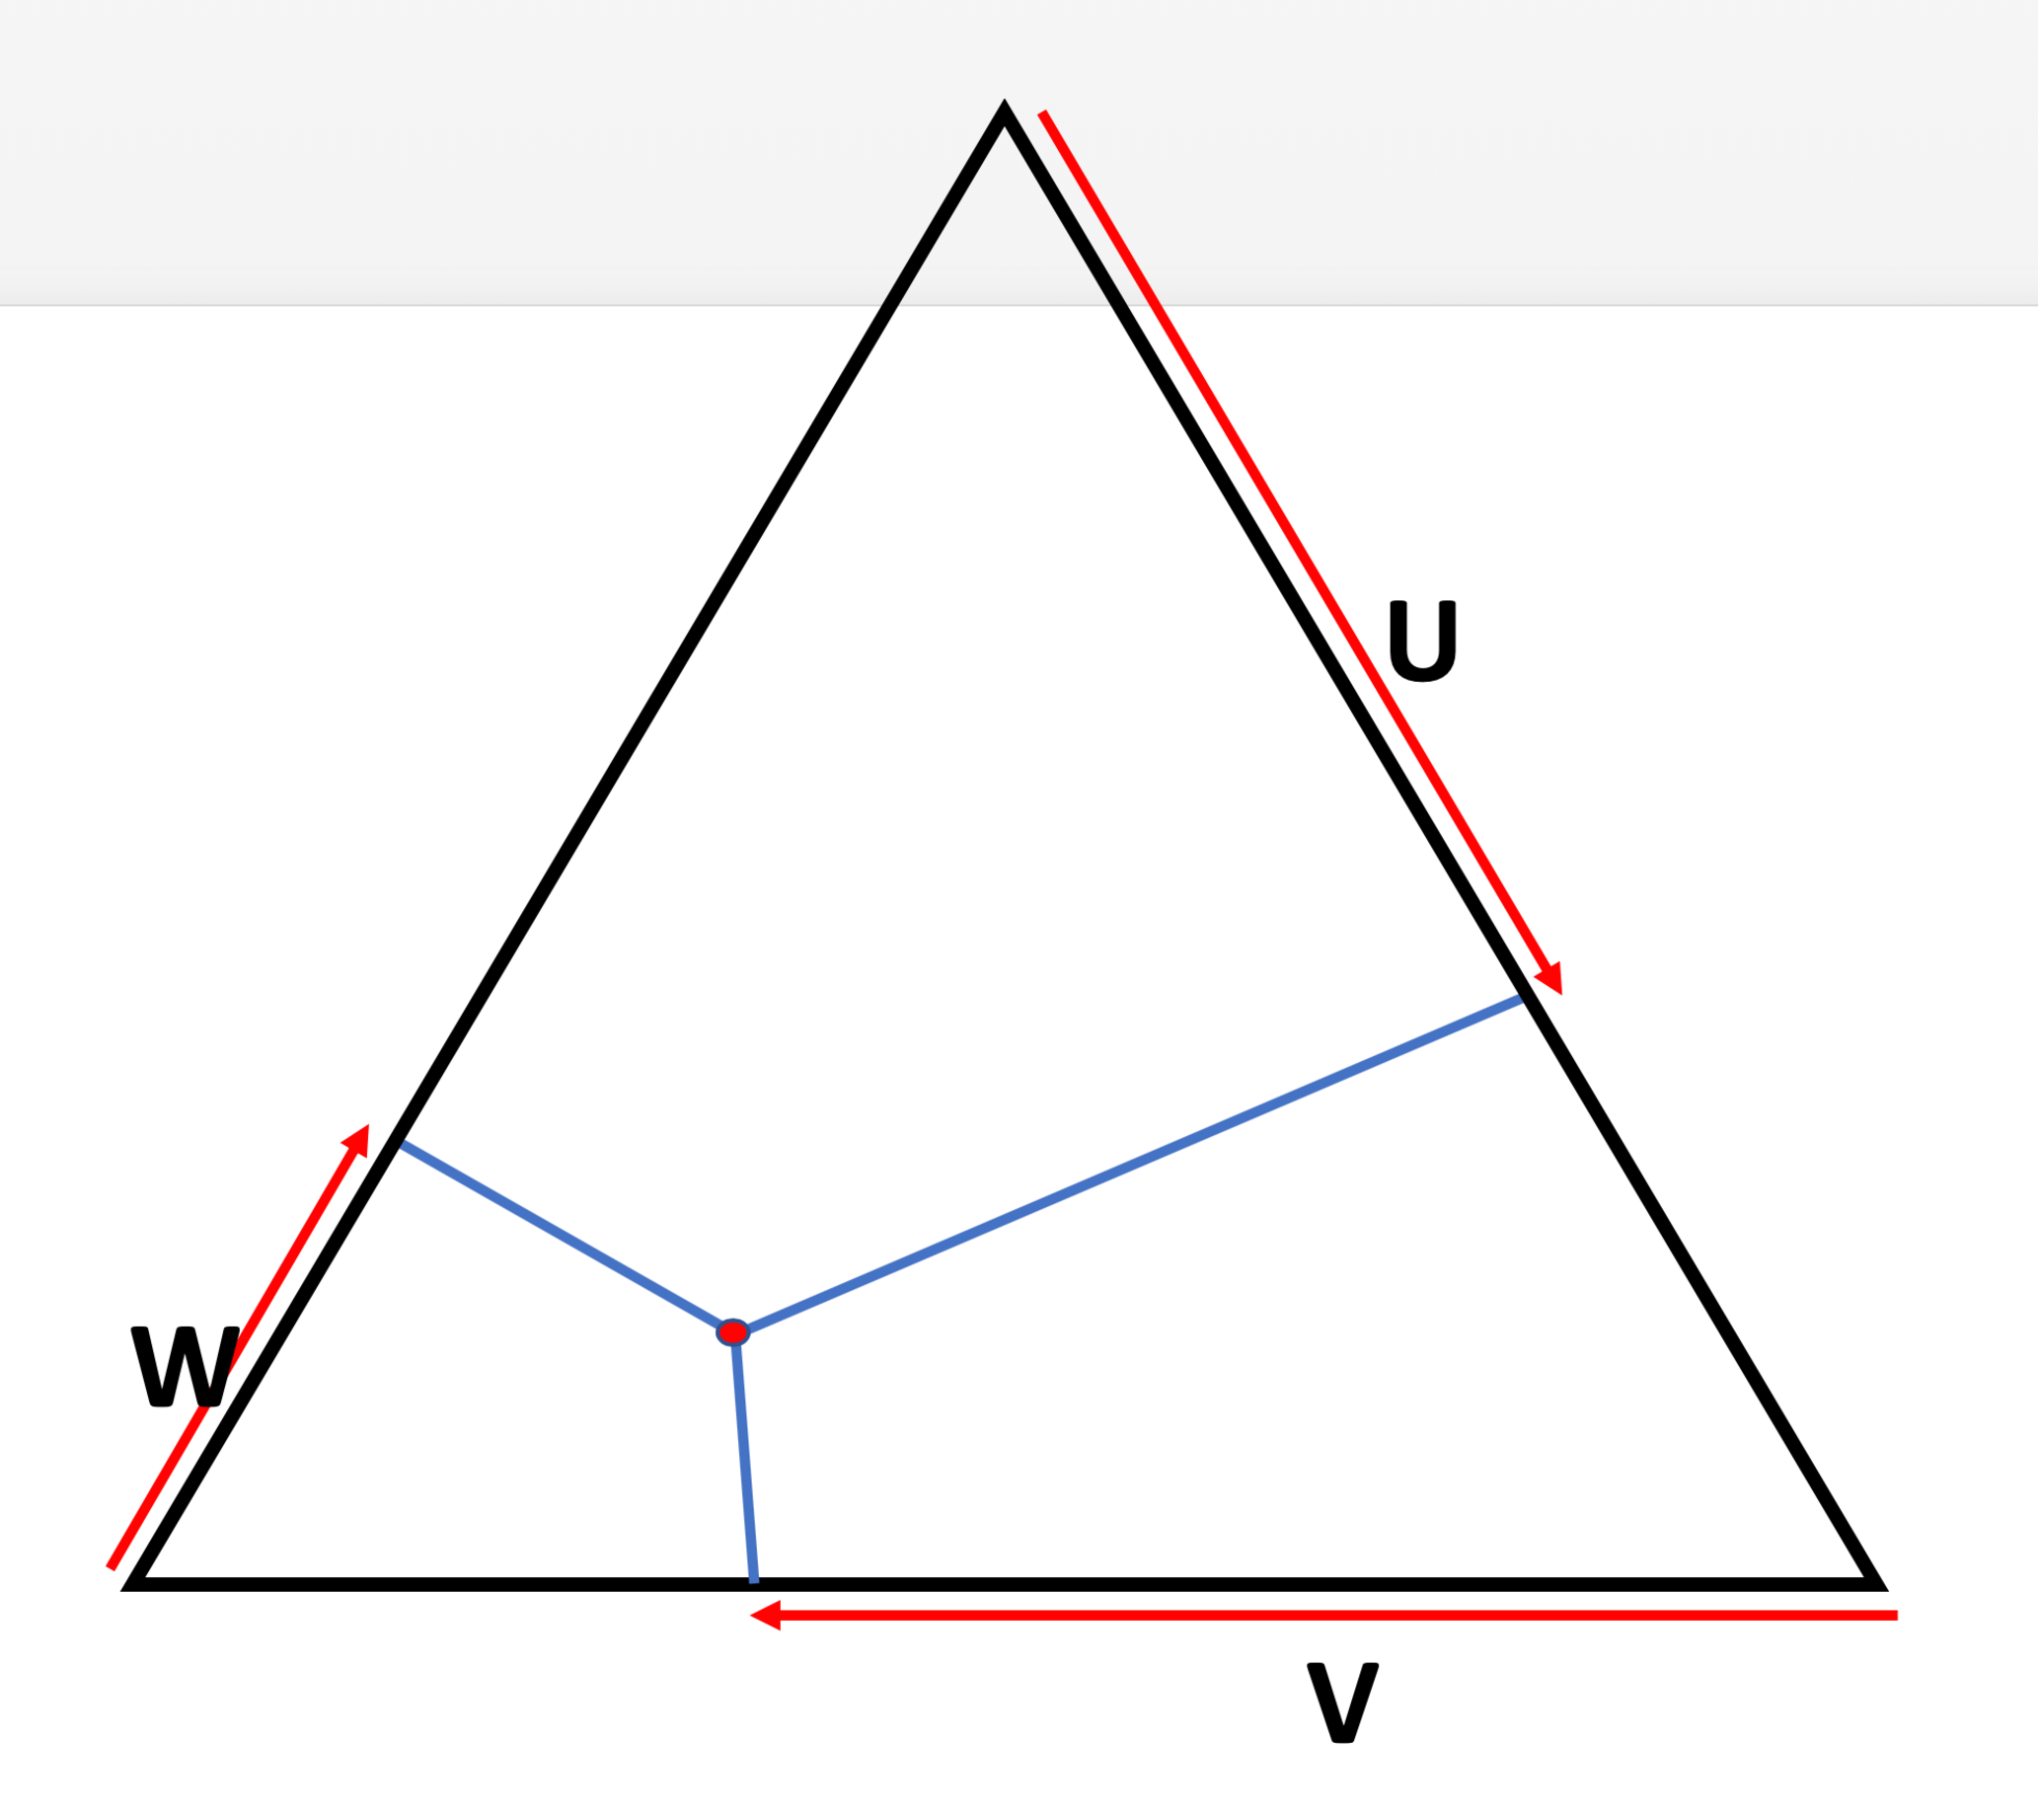
\includegraphics[width=7cm]{img/PCAL-EC.pdf}
		%\includegraphics{PCA.pdf}
		\caption{Cluster's reconstruction in the PCAL and EC calorimeters}
		\label{fig:PCAL}
	\end{center}
\end{figure} 


\subsubsection{Drift Chamber} sergey,ben
\label{sec:DC}

CLAS12 Drift Chamber (DC, ref) contains six superlayers, six layers in each superlayers, 112 wires in every layer. Trigger algorithm was designed as two-step process.

First it searches for segments in each of six superlayers, reporting 112-bit mask with bits set for segments found. Search for segments is conducted based on pre-loaded segment dictionary, generated by drift chamber simulation software based on internal superlayer wires location. In case if several segments found in the same location the one with maximum number of hits are kept. In theory the number of layers in segment must be equal to 6, and the number of hit wires in one segment can vary from 6 to 12 depending on track position and angle. On practice, the number of layers and hits in segment can be less because of drift chamber inefficiencies and broken wires, so threshold for segment finder in trigger logic was usually set to 4 and sometimes to 3 layers out of 6.

After segment search complete and six 112-bit masks are ready second step is performed. On that step pre-loaded road dictionary is used to identify possible track candidates (so-called road finding). Road disctionaries can be generated by Monte Carlo program or taken from the real data, both methods were used. At least five out of six superlayers are required to satisfy trigger condition. All found roads are reported to the Stage 2 every 16 ns. Reported information contains ... for geometry match on Stage 2.


\subsubsection{High Threshold Cherenkov Counter} sergey
\label{sec:HTCC}

CLAS12 High Threshold Cherenkov Counter (HTCC, ref) serves as one of primary components of electron trigger logic. It was specially designed to discriminate electrons from other charge particles. HTCC consists of 48 sections readout by PMTs connected to FADCs (Fig.~\ref{fig:multihitHTCC}). For trigger purposes 2x2 section sliding window is used to identify clusters. The cluster may include one, two, three or maximum four PMT's signals collecting the Cherenkov light from the adjacent mirrors as shown in  Fig.~\ref{fig:multihitHTCC}. Configuration parameters includes single channel energy threshold, cluster multiplicity threshold and cluster energy threshold. Resilts are reported to Stage 2 as 48-bit masks every 4 ns. FADC 'gain' configuration parameter allows energy calibration, making it possible to set energy thresholds in terms of the number of photoelectrons.


\begin{figure}[htp]
	\begin{center}
		\centering
		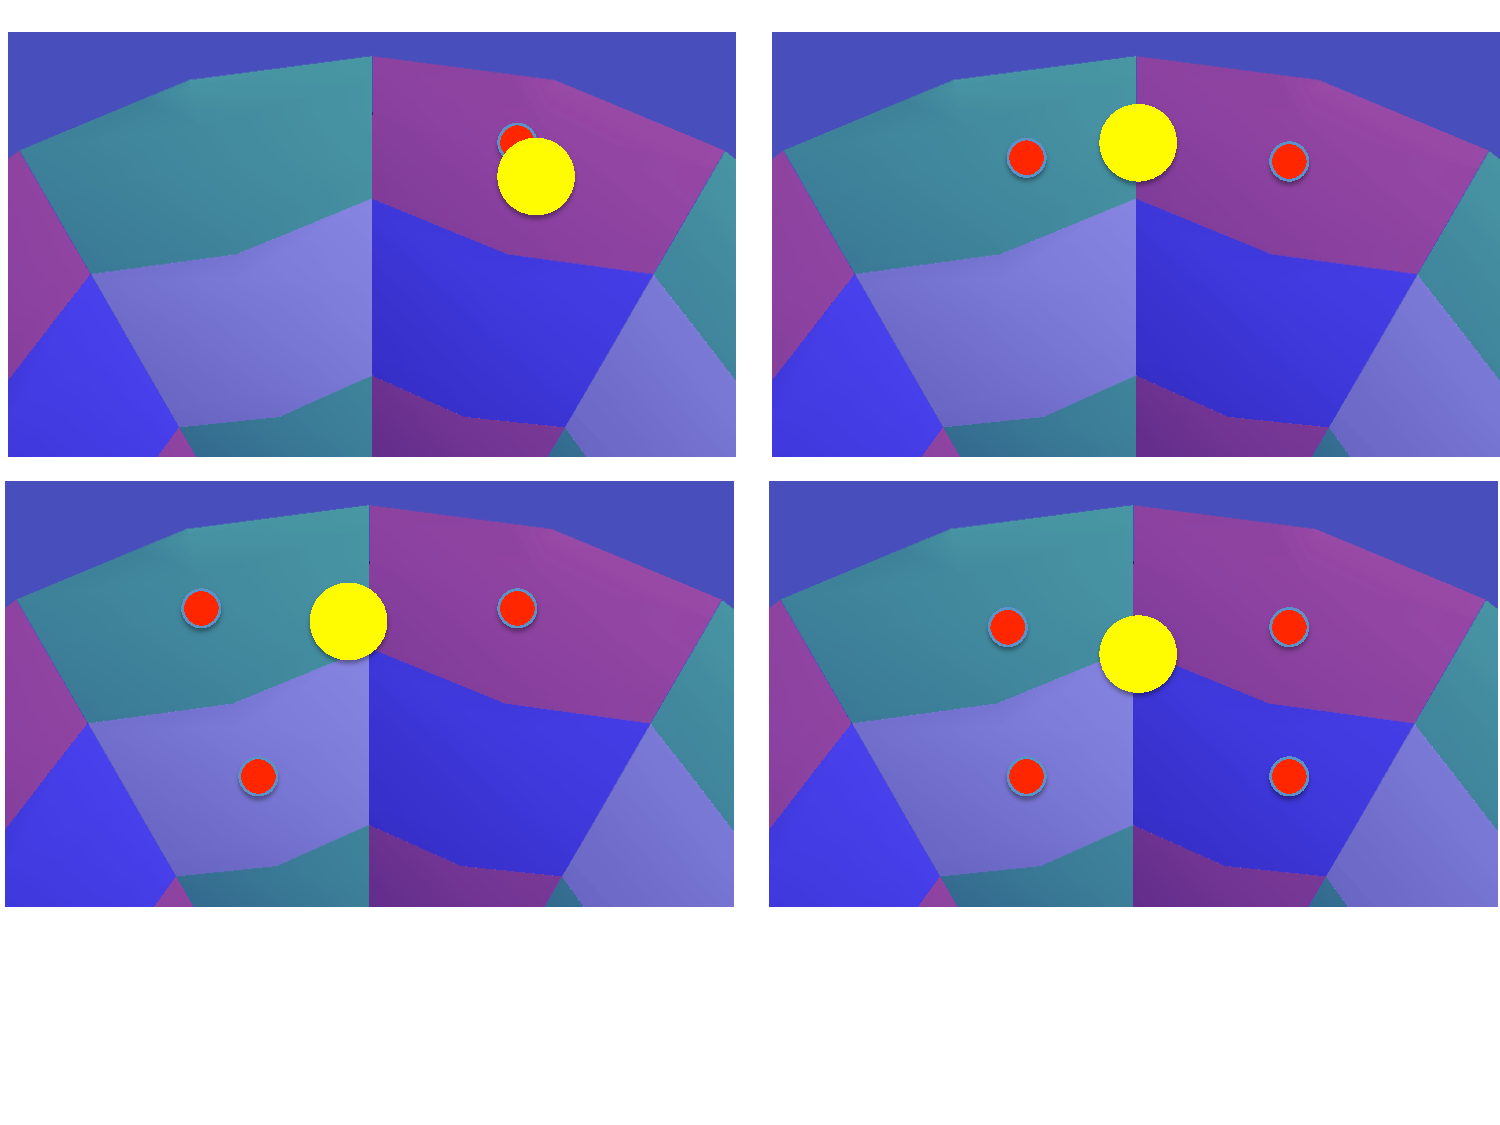
\includegraphics[width=8cm]{img/multiHits.pdf}
		\caption{Hits registered by HTCC (red circles) and reconstructed cluster position (yellow). They coincide for one hit clusters (top left plot) which has the lowest resolution.}
		\label{fig:multihitHTCC}
	\end{center}
\end{figure} 


\subsubsection{Forward Time-Of-Flight Counter} sergey

CLAS12 Forward Time-Of-Flight Counter (FTOF, ref) contains several layers of scintillating slabs, but only one layer is used by trigger logic. It contains 64 counters with PMT readout from both ends. When both end PMTs reports signal trigger system consider it as hit. 64-bit hit mask reported to the Stage 2 every 4 ns. Trigger logic configuration includes single channel energy threshold and threshold for SQRT(EleftxEright). FTOF participates in non-electron triggers such as muon trigger.


\subsubsection{Central Time-Of-Flight Counter} sergey

CLAS12 Central Time-Of-Flight Counter (CTOF, ref) consists of 48 scintillation slabs, surrounding target as barrel, with PMT readout from both ends. Its trigger logic is similar to FTOF one, with 48-bit mask reported every 4 ns.


\subsubsection{Neutron Detector} sergey

CLAS12 Neutron Detector (CND, ref) consists of three layers of scintillation slabs, installed behind CTOF, with 24 slabs per layer and 72 counters total. Its trigger logic is similar to FTOF/CTOF one, with 24-bit mask reported every 4 ns (usually inner layer only).


\subsubsection{Forward Calorimeter and Hodoscope} andrea,ben

CLAS12 Forward Tagger Calorimeter and Hodoscope trigger is designed to trigger on electrons at small forward angles. The calorimeters is a stack of 332 lead tunstage cystals connected to APDs which are readout by FADCs. The hodoscope consists of two layers each having 116 pixels (of two sizes) which matches the geometry of the calorimeter. The calorimeter trigger finds clusters by looking for a seed hit at each crystal location. If the deposited energy in a crystal is greater than the seed threshold and it is a local maximum in space (using 3x3 view) and time then it is considered a seed hit. For each seed hit a cluster is formed by summing all of the energies centered on the seed hit in a 3x3 view is for all hits time coincident with the seed hit (up to +/-16ns). The seed hit time, which due to timewalk is the earliest hit in the cluster, is used for the cluster timestamp providing 4ns resolution. The geometrically matched hodoscope pixels for both layers are checked for time coincident hits with the calorimeter seed hit and the cluster is tagged as having none, layer 1, layer 2, or both layers of hodoscope present. Found clusters are serialized and streamed over fiber links to the 2nd trigger stage where several programmable trigger cuts can discriminate clusters based on energy, charge, and multiplicty.

\subsection{Stage 2}

The stage 2 trigger collects data from stage 1 crates using fiber optics. Multiple SSP modules are used to collect stage 1 trigger streams and form subsystem coincidences for 6 identical forward detectors and central detectors (all separately). Each subsystem trigger stream goes through a programmable delay that provides 4ns resolution when deskewing to optimize the time coincidence. Next follows a programmable coincident window for each subsystem trigger stream, also 4ns step resolution, to ensure that different subdetector signals will remain stable long enough to form a time coincidence regardless of jitter due to particle time-of-flight, detector, and trigger jitter.

\begin{center}
	Stage 2 Specs\\
	\begin{tabular}{| l | l |}
		\hline \hline
		Name				& Specification	\\
		\hline
		Latency (Stage 1+2)		& 5$\mu$s	\\
		Jitter				& 4ns		\\
		Stage 2 trigger bits		& 8		\\
		Deskew range			& 4$\mu$s	\\
		Deskew step size		& 4ns	\\
		Coincidence window range	& 2$\mu$s	\\
		Deskew step size		& 4ns	\\
		\hline \hline
	\end{tabular}
\end{center}

The forward detectors in the trigger consist of FTOF, ECAL, PCAL, HTCC, and DC. A single SSP collects all forward dector trigger streams from a single sector of CLAS12. After the delay and concidence widths are applied to each input stream the input streams are copied to 8 programmable sector trigger bits. Each sector trigger bit contains a variety of trigger primitives and customizeable thresolds/cuts that can be taylored for a particular trigger type. Sector trigger bits are computed and sent to the final trigger stage 3.

\begin{center}
	Forward Detector Trigger Primitives\\
	\begin{tabular}{| l | l |}
		\hline \hline
		Primitive Name			& Trigger Bit Parameters	\\
		\hline
		PCU     			& Mask				\\
		FTOF    			& Mask				\\
		PCAL				& Cluster Emin, Emax		\\
		ECAL				& Cluster Emin, Emax		\\
		PCAL+ECAL			& Cluster Emin			\\
		HTCC				& Mask				\\
		{\bf Geometry Matched}		&				\\
		PCUxFTOF			& Bar match tolerance		\\
		PCALxDC				& Cluster Emin			\\
		\hline \hline
	\end{tabular}
\end{center}

The central detectors participating in the trigger consist of CTOF, CND, and FT. A single SSP collects all central detector trigger streams. After the delay and concidence widths are applied to each input stream the input streams are copied to 8 programmable central trigger bits. Each central trigger bit contains a variety of trigger primitives and customizeable thresolds/cuts that can be taylored for a particular trigger type. Central trigger bits are computed and sent to the final trigger stage 3 where all sector and central trigger bits arrive at the GTP to compute the global trigger bits.

\begin{center}
	Central Detector Trigger Primitives\\
	\begin{tabular}{| l | l |}
		\hline \hline
		Primitive Name			& Trigger Bit Parameters	\\
		\hline
		CND     			& Mask				\\
		CTOF    			& Mask				\\
		FT				& Cluster Emin, Emax, 		\\
						& Cluster Size, Hodoscope	\\
		{\bf Geometry Matched}		&				\\
		CNDxCTOF			& Bar match tolerance		\\
		\hline \hline
	\end{tabular}
\end{center}


\subsection{Stage 3} ben

The stage 3 trigger is the final stage and collects all sector and central trigger bit streams in a single module where they can be combined in a variety of ways to generate the global trigger bits used for reading out the DAQ. There are 32 independent trigger bits that can form a trigger based on any combination of sector and/or central trigger bits. Each trigger bit contains two sector trigger bit conditions (required to both be true) and a signle central trigger bit condition. Additionally each trigger bit contains 16bit prescaler, final pulse width, and scaler.

\begin{center}
	Stage 3 Specs\\
	\begin{tabular}{| l | l |}
		\hline \hline
		Name				& Specification	\\
		\hline
		Latency (Stage 1+2+3)		& 7$\mu$s	\\
		Jitter				& 4ns		\\
		Stage 3 trigger bits		& 32		\\
		Prescaler			& 0-65535	\\
		Trigger bit width		& 4ns-1$\mu$s	\\
		Pulse rate			& 0.05Hz-125MHz	\\
		\hline \hline
	\end{tabular}
\end{center}

An important part of stage 3 is the event builder allowing it to participate in event-by-event readout like front-end crates. Each time the CLAS12 DAQ is triggered the stage 3 GTP component will also build an event which contains the trigger bit decisions for all 32bit for a given programmable window related to the readout trigger time. This allows trigger bits to be run in ``tagging mode'' and is a powerful way to test trigger efficiency (using either a loose trigger or random trigger).